\documentclass[tikz,border=8pt]{standalone}

\usepackage[T1]{fontenc}
\usepackage{helvet}
\renewcommand{\familydefault}{\sfdefault}
\usetikzlibrary{arrows.meta,backgrounds,fit,positioning}

\definecolor{ink}{HTML}{253238}
\definecolor{line}{HTML}{526A72}
\definecolor{sourcefill}{HTML}{F4E7CF}
\definecolor{processfill}{HTML}{DDEFF2}
\definecolor{storefill}{HTML}{E0EAD2}
\definecolor{runtimefill}{HTML}{D9E8E6}
\definecolor{outputfill}{HTML}{F3DFA2}
\definecolor{supportfill}{HTML}{ECEFF1}
\definecolor{laneoffline}{HTML}{F7FAFA}
\definecolor{laneruntime}{HTML}{F6F8F3}

\begin{document}
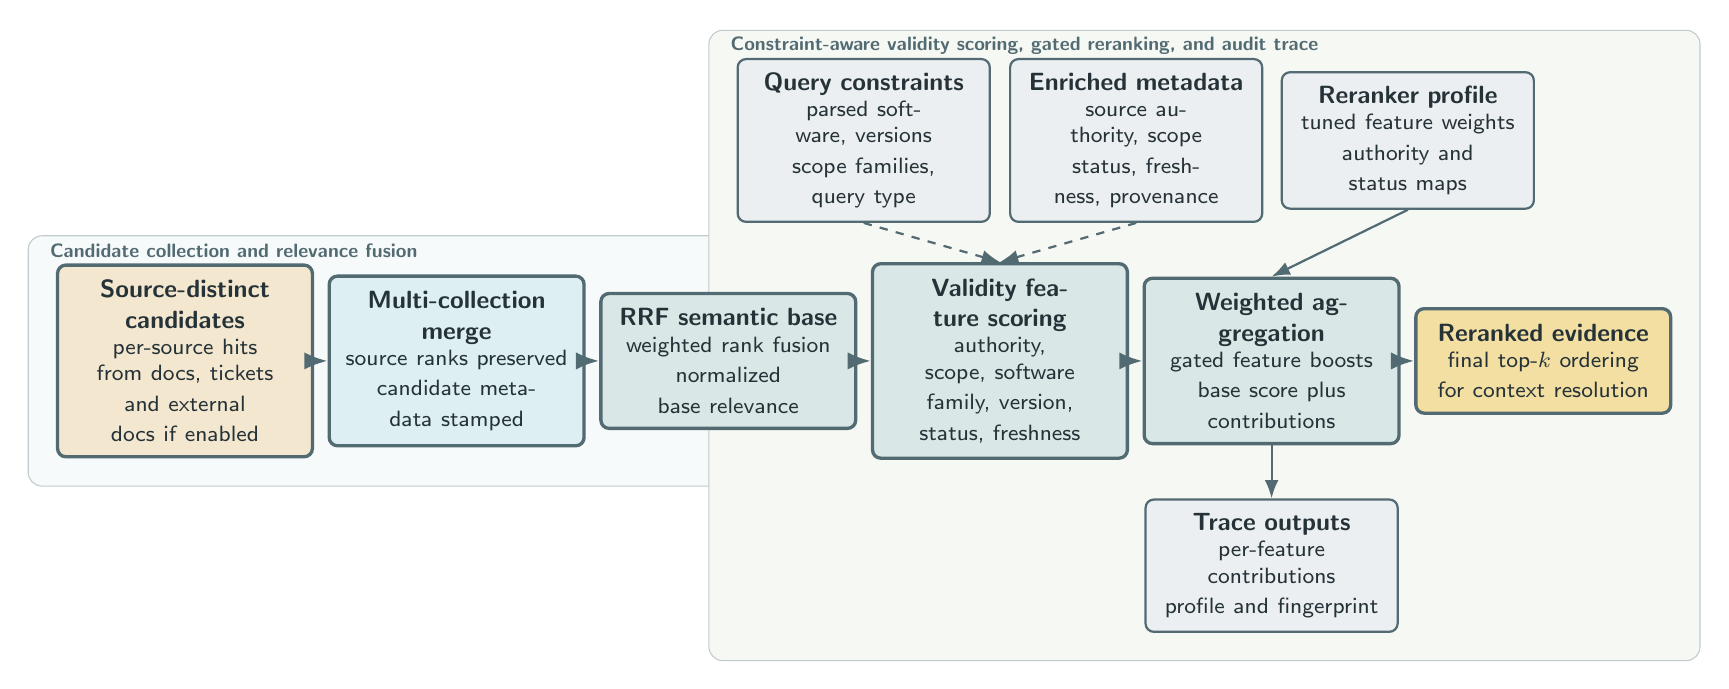
\begin{tikzpicture}[
  font=\small,
  text=ink,
  box/.style={
    draw=line,
    very thick,
    rounded corners=3pt,
    align=center,
    inner sep=5.5pt,
    minimum height=1.18cm,
    text width=2.85cm
  },
  compact/.style={
    draw=line,
    thick,
    rounded corners=3pt,
    align=center,
    inner sep=5pt,
    minimum height=1.00cm,
    text width=2.85cm
  },
  source/.style={box, fill=sourcefill},
  process/.style={box, fill=processfill},
  store/.style={box, fill=storefill},
  runtime/.style={box, fill=runtimefill},
  output/.style={box, fill=outputfill},
  support/.style={compact, fill=supportfill},
  arrow/.style={-Latex, very thick, draw=line},
  dataarrow/.style={-Latex, thick, draw=line},
  metaarrow/.style={-Latex, thick, dashed, draw=line},
  note/.style={font=\scriptsize, text=line, align=center},
  lane/.style={
    draw=line!35,
    rounded corners=5pt,
    fill=#1,
    inner sep=10pt
  }
]

% Candidate collection and semantic base
\node[source] (candidates) at (0,0.75) {\textbf{Source-distinct candidates}\\{\footnotesize per-source hits from docs, tickets\\and external docs if enabled}};
\node[process] (merge) at (3.45,0.75) {\textbf{Multi-collection merge}\\{\footnotesize source ranks preserved\\candidate metadata stamped}};
\node[runtime] (rrf) at (6.90,0.75) {\textbf{RRF semantic base}\\{\footnotesize weighted rank fusion\\normalized base relevance}};

\draw[arrow] (candidates) -- (merge);
\draw[arrow] (merge) -- (rrf);

% Validity-aware adjustment path
\node[runtime] (features) at (10.35,0.75) {\textbf{Validity feature scoring}\\{\footnotesize authority, scope, software\\family, version, status, freshness}};
\node[runtime] (aggregate) at (13.80,0.75) {\textbf{Weighted aggregation}\\{\footnotesize gated feature boosts\\base score plus contributions}};
\node[output] (reranked) at (17.25,0.75) {\textbf{Reranked evidence}\\{\footnotesize final top-$k$ ordering\\for context resolution}};

\draw[arrow] (rrf) -- (features);
\draw[arrow] (features) -- (aggregate);
\draw[arrow] (aggregate) -- (reranked);

% Support inputs and observability
\node[support] (constraints) at (8.62,3.55) {\textbf{Query constraints}\\{\footnotesize parsed software, versions\\scope families, query type}};
\node[support] (metadata) at (12.08,3.55) {\textbf{Enriched metadata}\\{\footnotesize source authority, scope\\status, freshness, provenance}};
\node[support] (weights) at (15.53,3.55) {\textbf{Reranker profile}\\{\footnotesize tuned feature weights\\authority and status maps}};
\node[support] (trace) at (13.80,-1.85) {\textbf{Trace outputs}\\{\footnotesize per-feature contributions\\profile and fingerprint}};

\draw[metaarrow] (constraints.south) -- (features.north);
\draw[metaarrow] (metadata.south) -- (features.north);
\draw[dataarrow] (weights.south) -- (aggregate.north);
\draw[dataarrow] (aggregate.south) -- (trace.north);

% Lane backgrounds
\begin{scope}[on background layer]
  \node[lane=laneoffline, fit=(candidates)(merge)(rrf)] (semanticlane) {};
  \node[lane=laneruntime, fit=(features)(aggregate)(reranked)(constraints)(metadata)(weights)(trace)] (validitylane) {};
\end{scope}

\node[note, anchor=west] at ([xshift=0.16cm,yshift=-0.20cm]semanticlane.north west) {\textbf{Candidate collection and relevance fusion}};
\node[note, anchor=west] at ([xshift=0.16cm,yshift=-0.20cm]validitylane.north west) {\textbf{Constraint-aware validity scoring, gated reranking, and audit trace}};

\end{tikzpicture}
\end{document}
